%Information relative au document
% !TEX encoding = MacOSRoman
\documentclass[a4paper,12pt]{report}


%Paquets
\usepackage[T1]{fontenc}
\usepackage[applemac]{inputenc}
\usepackage{xspace}
\usepackage[frenchb]{babel}
\usepackage{textcomp}
\usepackage{lmodern}
\usepackage{setspace}
\onehalfspacing
\usepackage{graphicx}
\usepackage{amsmath}
\usepackage{amsthm}
\usepackage{amssymb}
\usepackage{amsfonts}
%Pour faire un tableau de d\'eriv\'e
\usepackage{tikz,tkz-tab}
\usepackage{float}
\usepackage{here}
\usepackage[left=2cm,right=2cm,top=3cm,bottom=3cm]{geometry}
\usepackage{listings}
%Pour inclure du code
\lstset{numbers=left, numberstyle=\tiny, stepnumber=5, numbersep=5pt, language=Scilab, basicstyle=\small,frame=leftline,captionpos=b,linewidth=175mm,breaklines=true, commentstyle=\color{green},stringstyle=\color{red},identifierstyle=\ttfamily,keywordstyle=\color{blue}}

\newtheorem{definition}{Definition}


%D\'ebut du rapport
\begin{document}

%Page de garde
%\title{Rapport TP \no1 MT12}
%\author{Alexandre BALLET et Simon LAURENT}
%\date{Printemps 2016}

\thispagestyle{empty}


\includegraphics[scale=0.06]{logo_utc.png}

{\large

\vspace*{1cm}

\begin{center}

{\bf Rapport de MT12 : Techniques math\'ematiques de l'ing\'enieur \\ UNIVERSIT\'E DE TECHNOLOGIE DE COMPI\`EGNE}

\vspace*{1 cm}

\vspace*{1cm}

Printemps 2016

\vspace*{1cm}

\vspace*{1cm}
{\Large {\bf Alexandre BALLET et Simon LAURENT}}
\vspace*{2cm}

\vspace*{2 cm}
\end{center}

\flushleft{Sujet du rapport:\ \\
{\Large {\bf Transform\'ee de Fourier discr\`ete}}}

\vspace*{1 cm}
\flushleft{D\'epartement des \'etudiants :\ \\
{\Large {\bf  G\'enie Informatique}}}\\

\vspace*{1 cm}
\flushleft{Professeur :\ \\
{\Large {\bf M. Djalil KATEB}}}\\
}

\newpage
\null
\newpage
%Table des mati\`eres
\tableofcontents


%Questions 2.0 et 2.1
\chapter{D\'efinition de la DFT}

	%Question 2.0
	\section{D\'efinition}

	\begin{definition}
		On appelle transform\'ee de Fourier discr\`ete de la suite $(y_k),~k=0,~ldots,N-1$ la suite $(z_k)$ d\'efinie par 
		$$
		z_k=\cfrac{1}{N}\sum_{p=0}^{N-1}y_p\omega^{pk}
		$$
		o\`u $\omega=e^{-2i\frac{\pi}{N}}$. On notera $z[k]=DFT[f]k],~k=0,...,N-1$.
	\end{definition}

	Nous cherchons \`a montrer que

	\begin{equation}
		\sum_{k=0}^{N-1}\omega^{k(p-p')}=\left\{\begin{array}{lll} 0 &~\text{si}~&p\neq p'\\N&~\text{si}~&p=p'\end{array}\right.
		\label{11}
	\end{equation}

	D'une part, posons $p=p'$ :

	\begin{eqnarray*}
		\sum_{k=0}^{N-1}\omega^{k(p-p')}&=&\sum_{k=0}^{N-1}1\\
		&=&N\\
	\end{eqnarray*}

	D'autre part, posons $p\neq p'$ : 

	\begin{eqnarray*}
		\sum_{k=0}^{N-1}\omega^{k(p-p')}&=&\sum_{k=0}^{N-1}(\omega^{p-p'})^{k}\\
		&=&\frac{1-\omega^{(p-p')^{k}}}{1-\omega^{p-p'}}\\
		&=&\frac{1-e^{-2i\pi (p-p')}}{1-e^{-2i\frac{\pi}{N}(p-p')}}\\
		&=&\frac{1-e^{-2i\pi k}}{1-e^{-2i\frac{\pi}{N}(p-p')}}\qquad,\;\text{o\`u}\;k\,\in\,\pmb{\mathbb{Z}}\\
		&=&\frac{1-1}{1-e^{-2i\frac{\pi}{N}(p-p')}}\\
		&=&0\\
	\end{eqnarray*}

	Nous cherchons ensuite \`a montrer que $B=\sqrt{N}A$ est une matrice unitaire, c'est-\`a-dire :

	\begin{equation}
		\overline{B^{T}}B=I\qquad,\;\text{o\`u I est la matrice identit\'e}\\
	\end{equation}

	\begin{eqnarray*}
		B&=&\sqrt{N}\cfrac{1}{N}\left(
								\begin{array}{lllll}
									1&1&1& \ldots&1\\
									1&\omega&\omega^2&\ldots&\omega^{N-1}\\
									1&\omega^2&\omega^4&\ldots&\omega^{2(N-1)}\\
									1&\omega^3&\omega^6&\ldots&\omega^{3(N-1)}\\
									\vdots&\vdots&\vdots&&\vdots\\
									1&\omega^{N-1}&\omega^{2(N-1)}&\ldots&\omega^{(N-1)^2}
								\end{array}
								\right)\\
		\overline{B^{T}}B&=&\cfrac{\sqrt{N}}{N}\left(
								\begin{array}{lllll}
									1&1&1& \ldots&1\\
									1&(\overline{\omega})&(\overline{\omega})^2&\ldots&(\overline{\omega})^{N-1}\\
									1&(\overline{\omega})^2&(\overline{\omega})^4&\ldots&(\overline{\omega})^{2(N-1)}\\
									1&(\overline{\omega})^3&(\overline{\omega})^6&\ldots&(\overline{\omega})^{3(N-1)}\\
									\vdots&\vdots&\vdots&&\vdots\\
									1&(\overline{\omega})^{N-1}&(\overline{\omega})^{2(N-1)}&\ldots&(\overline{\omega})^{(N-1)^2}
								\end{array}
								\right)
							\cfrac{\sqrt{N}}{N}\left(
								\begin{array}{lllll}
									1&1&1& \ldots&1\\
									1&\omega&\omega^2&\ldots&\omega^{N-1}\\
									1&\omega^2&\omega^4&\ldots&\omega^{2(N-1)}\\
									1&\omega^3&\omega^6&\ldots&\omega^{3(N-1)}\\
									\vdots&\vdots&\vdots&&\vdots\\
									1&\omega^{N-1}&\omega^{2(N-1)}&\ldots&\omega^{(N-1)^2}
								\end{array}
								\right)\\
						&=&\cfrac{1}{N}(1+(\overline{\omega})^{p-1}(\omega)^{p'-1}+...+(\overline{\omega})^{(N-1)(p-1)}(\omega)^{(N-1)(p'-1)})\\
						&=&\cfrac{1}{N}(1+(\omega)^{p'-p}+...+(\omega)^{(N-1)(p'-p)})\\
						&=&\cfrac{1}{N}\sum_{k=0}^{N-1}\omega^{k(p'-p)}\\
						&=&\cfrac{1}{N}N\qquad,\;\text{d'apr\`es \eqref{11}}\\
						&=&1\\
	\end{eqnarray*}

	D'o\`u $B=\sqrt{N}A$ est une matrice unitaire.

	Nous cherchons \`a pr\'esent $A^{-1}$ :

	\begin{eqnarray*}
		\overline{B^{T}}B&=&I\\
		N\overline{A^{T}}A&=&I\\
		A^{-1}&=&N\overline{A^{T}}\\
		A^{-1}&=&\overline{\left(
								\begin{array}{lllll}
									1&1&1& \ldots&1\\
									1&\omega&\omega^2&\ldots&\omega^{N-1}\\
									1&\omega^2&\omega^4&\ldots&\omega^{2(N-1)}\\
									1&\omega^3&\omega^6&\ldots&\omega^{3(N-1)}\\
									\vdots&\vdots&\vdots&&\vdots\\
									1&\omega^{N-1}&\omega^{2(N-1)}&\ldots&\omega^{(N-1)^2}
								\end{array}
								\right)^{T}}\\
	\end{eqnarray*}

	$A^{-1}$ est la matrice associ\`ee \`a la transformation inverse de la DFT, que l'on peut retrouver :

	\begin{equation}
		z'_k=\sum_{p=0}^{N-1}y_p\omega^{-pk}\qquad,\;\text{o\`u}\;\omega=e^{-2i\frac{\pi}{N}}
	\end{equation}


	%Question 2.1
	\section{DFT d'une fonction}

	Soit f d\'efinie sur une p\'eriode T (p\'eriodique de p\'eriode T) et soit $(y_{k})$ une suite d'\'echantillons de $f$ en N points uniform\'ement r\'epartis sur une p\'eriode. La DFT de $f$ d'ordre $N$ est l'application qui associe \`a la suite $(y_{k})_{k=0,...,N-1}$ la suite constitu\'ee de la DFT appliqu\'ee au vecteur $y = (y_{k})_{k=0,...,N-1}$. On note $(DFT[f](k))_{0,...,N-1}$ la suite obtenue et $iDFT$ sa r\'eciproque.

	Nous cherchons \`a montrer que l'on peut approcher le coefficient de Fourier $c_{n}$ \`a partir de l'approximation de l'int\'egrale la d\'effinissant par une somme de Riemann.

	D'apr\`es la d\'efinition de $c_{n}$ on a : \[c_{n}=\frac{1}{T}\int_{0}^{T}f(t)e^{-2i\pi \frac{n}{T}t}dt\]

	Si nous discr\`etisons $f(t)$ en divisant une p\'eriode $T$ en $N$ segments, on obtient :

	\begin{eqnarray*}
		c_{n}&=&\frac{1}{T}\int_{0}^{T}f(t)e^{-2i\pi \frac{n}{T}t}dt\\
		&=&\frac{1}{T}\sum_{k=0}^{N-1}f(t_{k})e^{-2i\pi \frac{n}{T}k\frac{T}{N}}\frac{T}{N}\\
		&=&\frac{1}{N}\sum_{k=0}^{N-1}y_{k}e^{-2i\pi n\frac{k}{N}}\\
		&=&\frac{1}{N}\sum_{p=0}^{N-1}y_{p}e^{-2i\pi n\frac{p}{N}}\\
		&=&\frac{1}{N}\sum_{p=0}^{N-1}y_{p}\omega^{np}\\
	\end{eqnarray*}

	D'o\`u \[c_{k}=\frac{1}{N}\sum_{p=0}^{N-1}y_{p}\omega^{pk}\]

	Nous pouvons en d\'eduire que la DFT d'une suite $(y_{k})$ est \'equivalent au coefficient de Fourier $c_{k}$ de cette s\'erie.
	
%Question 2.2
\chapter{Une famille de fonctions tests}
	
	\section{Proc\'edure Scilab}
\begin{lstlisting}
_T = 1 
_alpha=1/3


function [y] = f(x)
    x=[pmodulo(x + _T/2,_T) - _T/2]
    y = zeros(x)
    for i=1:length(x)
        if (x(i) <_T*_alpha/2 & x(i)>-_T*_alpha/2) then
            y(i)=1
        
         else
            y(i) = 0
        end
    end
endfunction

N = 32


x=[-3*_T/2:_T/N:3*_T/2]
scf(0)
clf
plot(x,f(x),'xr')
		\end{lstlisting}\newpage

\begin{center}
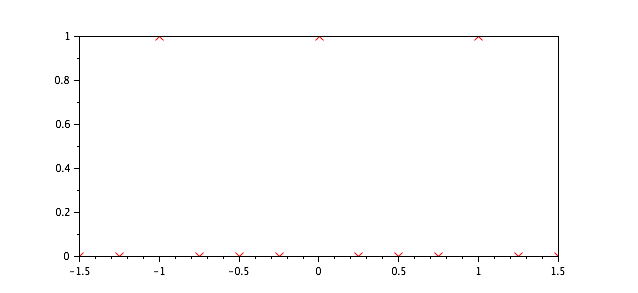
\includegraphics[scale=0.5]{FigEx2_2N4.png}\\
\caption{\textit{Repr\'esentation pour N=4}}
\end{center}

\begin{center}
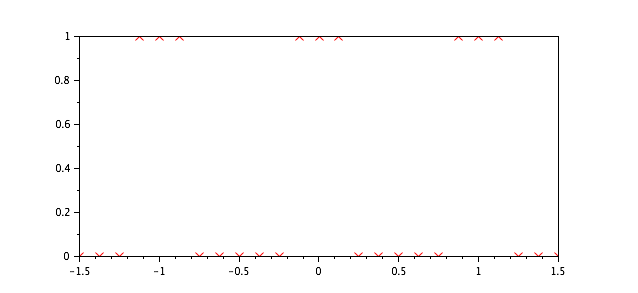
\includegraphics[scale=0.5]{FigEx2_2N8.png}\\
\caption{\textit{Repr\'esentation pour N=8}}
\end{center}

\begin{center}
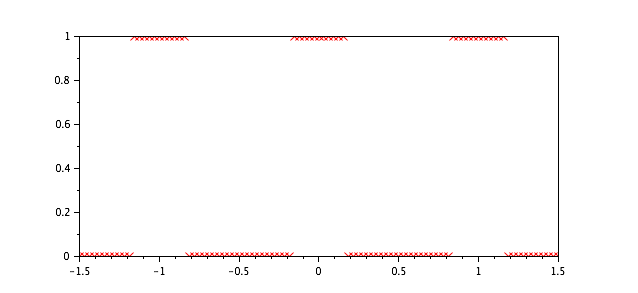
\includegraphics[scale=0.5]{FigEx2_2N32.png}\\
\caption{\textit{Repr\'esentation pour N=32}}
\end{center}

%Questions 2.3 et 2.4
\chapter{Applications de la DFT}

	%Question 2.3
	\section{Approximation des coefficients de Fourier}
\begin{lstlisting}
//****************
//Calcul de la DFT
//****************
f0=312;
N=1024;//num�risation
for Fe=2000:-50:500
    //instants de mesure
    t=(0:N-1)/Fe;
    //signal temporel
    x=sin(2*%pi*f0*t)+sin(2*%pi*t*500)
    //calcul de la FFT du signal;
    X=fft(x);
    [mx,p]=max(abs(X(1:N/2)));
    //trace du spectre entre -Fe/2 et Fe/2
    f=(-fix(N/2):N-fix(N/2)-1)/N*Fe;
    figure(0)
    //Desactivation des commandes graphiques
    drawlater;
    clf();
 title(['spectre sinusoide de freq'+string(f0)+'Hz numer a '+string(Fe)+'Hz'])
h=gce();
plot(f,abs(fftshift(X)))
drawnow
//xpause(200000)
xclick
end
\end{lstlisting}\newpage

	%Question 2.4
	\section{R\'esolution fr\'equentielle de signaux}

		\subsection{Mise en jambes}

		\subsection{Exercice}

%Question 2.5
\chapter{DFT et convolution}

%Question 2.6
\chapter{Ph\'enom\`ene de Gibbs}

%Question 2.8
\chapter{Effet du fen\^etrage}

%Table des figures
\listoffigures

\end{document}